\documentclass[a4paper,12pt]{article}
\usepackage[english]{babel}
\usepackage[utf8]{inputenc}
\usepackage{amssymb}
\usepackage{amsmath}
\usepackage{mathtools}
\usepackage{listings, lstautogobble}
\usepackage{tikz}
\usepackage{graphicx}
\graphicspath{ {./images/} }
\usepackage{xcolor}
\usepackage{array}
\usepackage{hyperref}
\hypersetup{
    colorlinks=true,
    linkcolor=blue,
    filecolor=magenta,      
    urlcolor=cyan,
}

\urlstyle{same}

\definecolor{RoyalBlue}{cmyk}{1, 0.50, 0, 0}

% Code listing init
\lstset{
  keywordstyle=\color{RoyalBlue},
  basicstyle=\scriptsize\ttfamily,
  commentstyle=\ttfamily\itshape\color{gray},
  stringstyle=\ttfamily,
  showstringspaces=false,
  breaklines=true,
  frameround=ffff,
  frame=single,
  language=bash,
  rulecolor=\color{black},
  autogobble=true
}

\pagestyle{headings}

\begin{document}

\markright{Entropass}
%%%%%%%%%%%%%%%%%%%%%%%%%%%%%%%%%%%%%%%%%%%%%%%%%%%%%%%%%%%%%%%%%%%%%%%%%%%%%%%%
%%%%%%%%%%%%%%%%%%%%%%%%%%%%%%%%%%%%%%%%%%%%%%%%%%%%%%%%%%%%%%%%%%%%%%%%%%%%%%%%
%%%%%%%%%%%%%%%%%%%%%%%%%%%%%%%%%%%%%%%%%%%%%%%%%%%%%%%%%%%%%%%%%%%%%%%%%%%%%%%%
\begin{titlepage}
  % \maketitle
  \begin{center}
    \vspace*{1cm}

    \Huge
    \textbf{Research Report}

    \vspace{0.5cm}
    \LARGE
    Entropass

    \vspace{1.5cm}

    \textbf{Jochem Stevense}

    \vfill

    A research report presented for the design \& implementation of Entropass

    \vspace{0.8cm}

    % \includegraphics[width=0.4\textwidth]{imagefile}

    \Large
    Embedded Systems Engineering\\
    Flexible Project\\
    Hogeschool van Arnhem en Nijmegen\\
    Ton Ammerlaan, Remko Welling\\
    The Netherlands\\
    2021\\
    Version 0.1
  \end{center}
\end{titlepage}

\thispagestyle{plain}
\begin{center}
    \Large
    \textbf{Research Report}
        
    \vspace{0.4cm}
    \large
    Entropass
        
    \vspace{0.4cm}
    \textbf{Jochem Stevense}
       
    \vspace{0.9cm}
    \textbf{Abstract}
  \end{center}
  put some text here
  \newpage
%%%%%%%%%%%%%%%%%%%%%%%%%%%%%%%%%%%%%%%%%%%%%%%%%%%%%%%%%%%%%%%%%%%%
  
\section*{Preface}
\newpage
  
%%%%%%%%%%%%%%%%%%%%%%%%%%%%%%%%%%%%%%%%%%%%%%%%%%%%%%%%%%%%%%%%%%%%%%%%%%%%%%%%
\tableofcontents

\newpage
%%%%%%%%%%%%%%%%%%%%%%%%%%%%%%%%%%%%%%%%%%%%%%%%%%%%%%%%%%%%%%%%%%%%%%%%%%%%%%%%
\section{Introduction}
\label{ch:intro}
This research report has been created for the Hogeschool van Arnhem en Nijmegen as part of the Bachelor Flexible Project of Jochem Stevense and investigates the possibilities of developing a tool to efficiently guess for passwords, targeting a single specific person. The purpose of such a tool is to show users the vulnerabilities introduced by using memorable passwords and to generate wordlists to be used for ethical hacking and penetration testing purposes.\\

Wordlists are used by threat actors to perform dictionary attacks on services that require authentication, parsing through a list of words and trying to login, using these words as passwords. The same can be done with usernames, although usernames are generally easier to discover, depending on the service to authenticate to.\\
Most of the wordlists available are simply a compilation of previously discovered passwords, resulting from data breaches, and often hold the most used ones or the ones found in a specific data breach. This can prove useful when targeting a large number of users, since it is likely that one of these users will use a password that is included in the list. However, when targeting a single user, the odds of the password being included in such a list can be small. The reason for this is that many users use personalised passwords to be able to memorise the credentials. Although these personalised passwords are unlikely to be included in a general wordlist, they are often not hard to guess, when personal information about a target user is known.\\
This research aims to gain insight into what functionality a password wordlist generating tool would need, to be able to guess these personalised passwords for a single user. To reach this goal, the following research question has been defined:\\

\textit{What functionalities should a password wordlist generating tool have to be able to utilise standard password practices when targeting a single, specific user?}

The main research question has been divided into several sub-questions. These sub-questions are the following:

\begin{itemize}
\item \textit{What are standard password formats?}
\item \textit{What personal information is relevant for password guessing?}
\item \textit{How can the processed information be structured efficiently, to allow for efficient dictionary attacks?}
\item \textit{How can the program remain up to date with changing password practices?}
\end{itemize}

This research will consist of a combination of qualitative and quantitative research to find the most used password formats, used personal information for passwords, how the information can be structured and how to remain up to date with changing password practices. Desk research will be used to find the most used password formats, by gathering leaked passwords, publically available and analysing the passwords for the formats, and most used characters. The found passwords will also be analysed to detect personal information embedded into the passwords. Once this information is found, field research will be used to test the structuring of the data and how to analyse the data automatically and keep up with changing password practices.

\newpage
\section{Research}

\subsection{Theoretical Framework}
Ma, Campbell Tran and Kleeman \cite{bib:entro} mention that password entropy, used to indicate password strength, is loosely defined and mention that the calculation of this entropy is an inadequate indicator to password strength. Password strength is not only defined by the used character library and length, but is also relative to the attacker. Entropy calculations might indicate a password to be very strong, even though the actual entropy is effectively very low if an attacker has accurate ideas on what this password might be.\\

Chou, Lee, Yu, Lai, Huang and Hsueh \cite{bib:pform} define password formats to have certain lengths, a combination of characters, and a pattern in the order of the characters and have proven so with the help of machine learning tools to learn these patterns and reproduce passwords using these patterns. This information allows for a clear direction for the analysing of password formats.

\subsection{Methodology}
The methodology deals with the methods, used to answer the sub-questions and the main question, formulated in chapter \ref{ch:intro}. Firstly, the sub-questions will be handled, after which the main research question will be dealt with.

\begin{itemize}
\item \textit{What are standard password formats?}\\
  To answer this question, desk research will be conducted, using online resources, such as leaked data/passwords, to create a list of formats, as used by users in the breach. The formats will be sorted in a list of most used to least used. The passwords will also be analysed for most used characters. This will be done automatically by using a Python script, which will be written specifically for the use of this research. The script will be made available for interested parties with the final project.
  
\item \textit{What personal information is relevant for password guessing?}\\
  Passwords are often based on personal information to make them easier to memorise. This personal information should be mapped to categories, to determine what a person is most likely to use for a memorable password. This will be done by desk research. This desk research will involve the use of the earlier mentioned word-lists from data breaches and analysing these manually to determine what categories are popular amongst users. Categories might involve aspects like, relationships, date of birth, pet names, etc.
  
\item \textit{How can the processed information be structured efficiently, to allow for efficient dictionary attacks?}
  To be able to answer this question, field research will be conducted to test different structures and determine which is most efficient in terms of finding the password as fast as possible. Several test scripts will be used to determine which structure is most efficient for a dictionary attack.

\item \textit{How can the program remain up to date with changing password practices?}
  This question will be answered by looking into sources of information for password practices, after which possibilities will be researched for gathering this information and analysing it in an automated way.
\end{itemize}

\subsection{Results}

The results of the research will be handled per question, firstly dealing with the sub-questions. The results are listed in this paragraph. The conclusions from these results will be dealt with in the Conclusions chapter.

\subsubsection{What are standard password formats?}

To be able to determine patterns in passwords, password formats have been researched. The formats have been defined as the combination of password length, used characters (differentiating between lower case alphabetical, higher case alphabetical, digits and special characters) and the positions of the used characters. To determine the most used password formats, several password files from Daniel Miessler's Seclists \cite{bib:seclists} have been used for analysis, with the help of custom Python scripts. These password files have been the results of disclosed data-breaches and are/were real passwords. The total number of used passwords is 37,045 (thirty seven thousand forty five), and the used files are listed in the Appendices \ref{app:pwordfile}. The total number of characters in the combined files is 294,028.\\

Figure \ref{fig:pform} shows the results of the password analysis, with the X-axis being populated with the discovered password formats, and the Y-axis indicating the number of times these formats have been found. The password formats contain a combination of $d$, $c$, $C$ and $s$. These character have the following meaning:
\begin{itemize}
\item $d=$Digit ($1,2,3,4,...$)
\item $c=$Lower-case Alphabetical character ($a,b,c,d,e,...$)
\item $C=$Higher-case Alphabetical character ($A,B,C,D,E,...$)
\item $s=$Special character ($',/,?,!,...$)
\end{itemize}

\begin{figure}[!ht]
  \centering
  \hspace*{-5.4cm}
  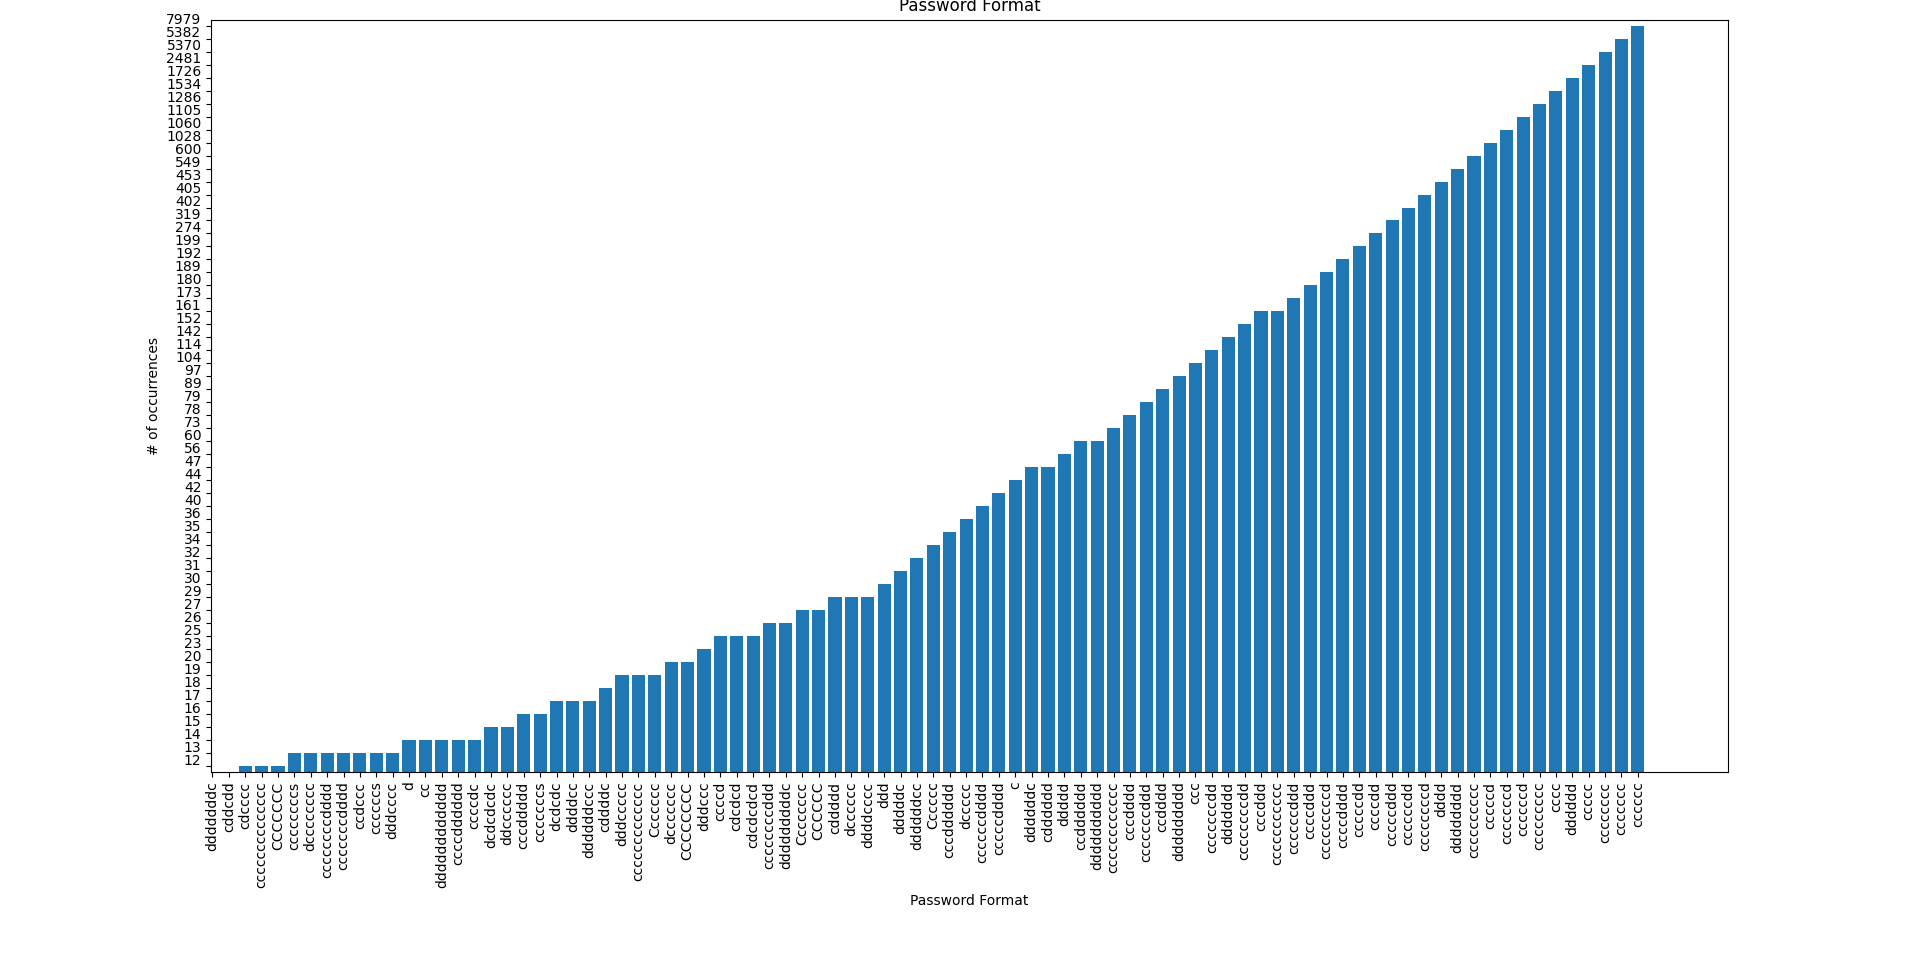
\includegraphics[width=1.8\textwidth]{password_formats}
  \caption{Password Format}
  \label{fig:pform}
\end{figure}

Notable from figure \ref{fig:pform} is that the top four (right most) password formats all consist of lower-case characters and the top seven consist of only one type of character, being lower-case alphabetical characters or digits. Looking further towards the left of the X-axis, this trend mostly holds, with only few combinations with at most two of the four types of characters. More than two types has not been discovered in the data sets. Overall, the lower-case alphabetical characters seem most popular, followed by digits.\\

Further analysis of the passwords can be seen in figure \ref{fig:pchar}. This graph confirms the statement that lower-case alphabetical characters are most popular, followed by digits. Only about halfway on the X-axis do more upper-case alphabetical characters and special characters appear, having at most about 1,200 occurrences in about 294,028 characters.

\begin{figure}[!ht]
  \centering
  \hspace*{-5.4cm}
  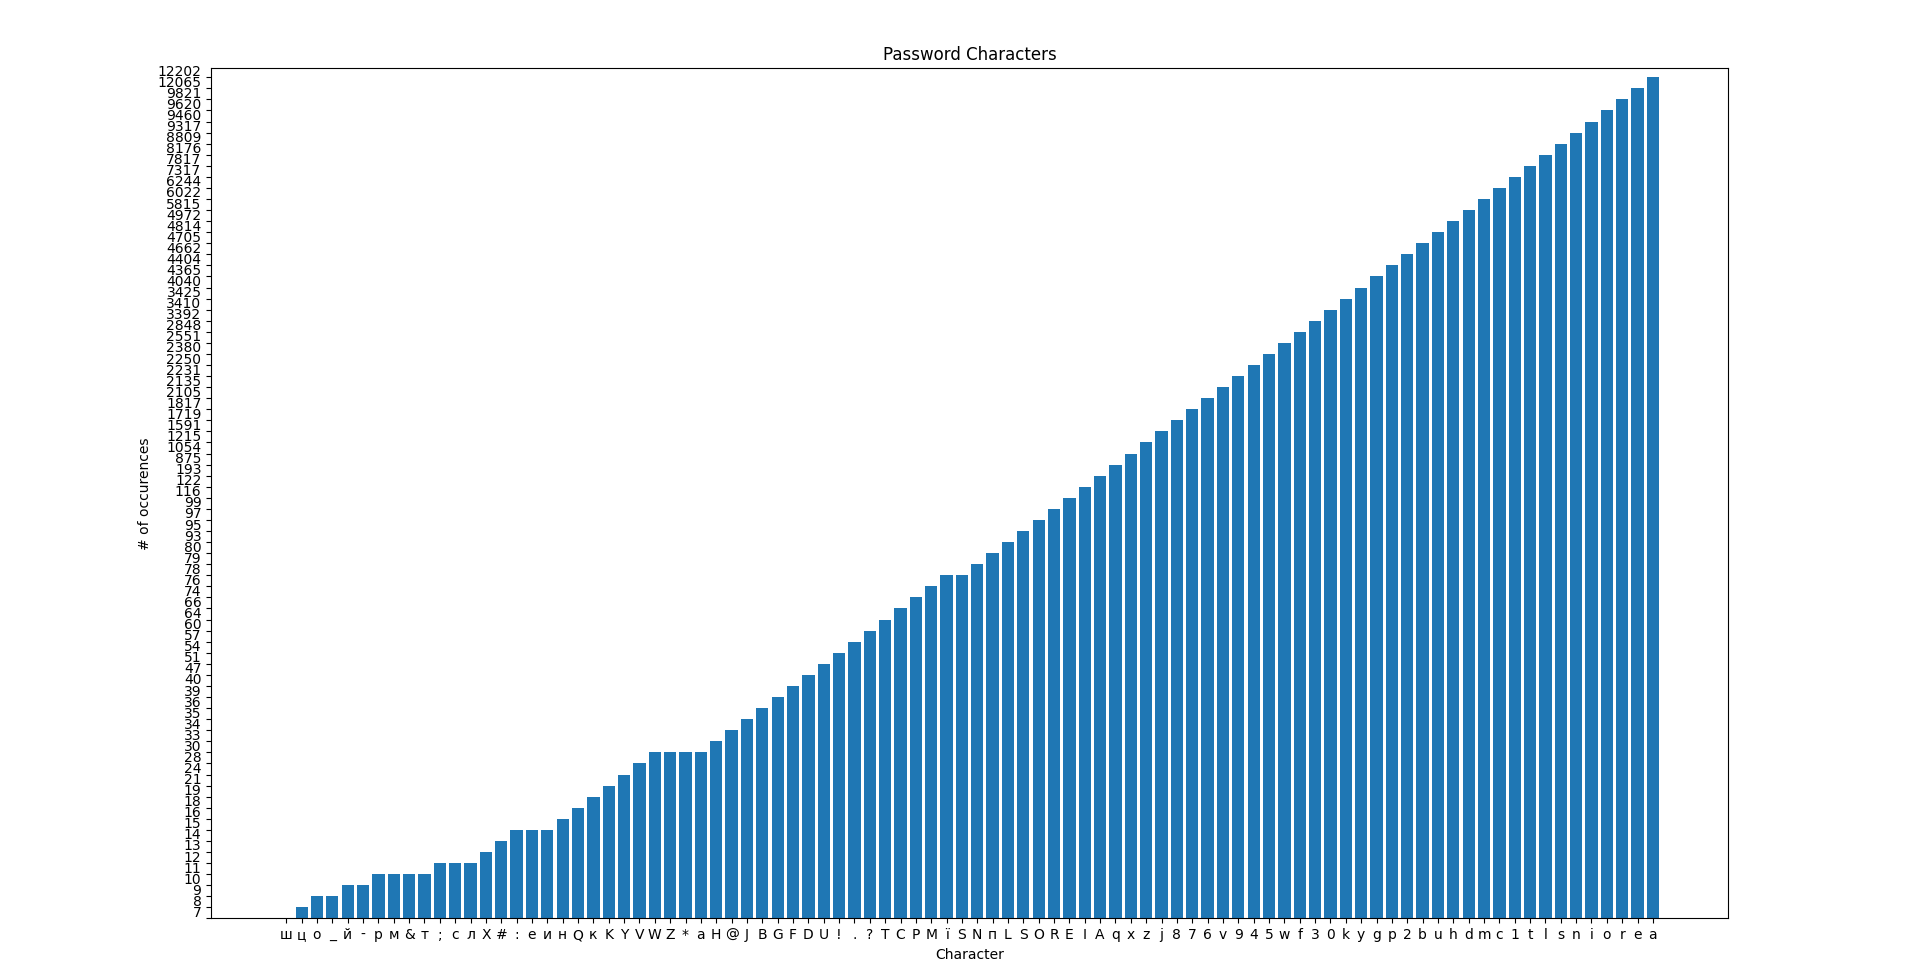
\includegraphics[width=1.8\textwidth]{password_chars}
  \caption{Character Usage}
  \label{fig:pchar}
\end{figure}

Focusing more on the length of the passwords, figure \ref{fig:plen} shows the most used password lengths. Perhaps unsurprisingly, the most used length of six is far from being the longest in the graph. Furthermore, the six most occurring lengths are all under 10, with 10 being the seventh most occurring.

\begin{figure}[!ht]
  \centering
  \hspace*{-5.4cm}
  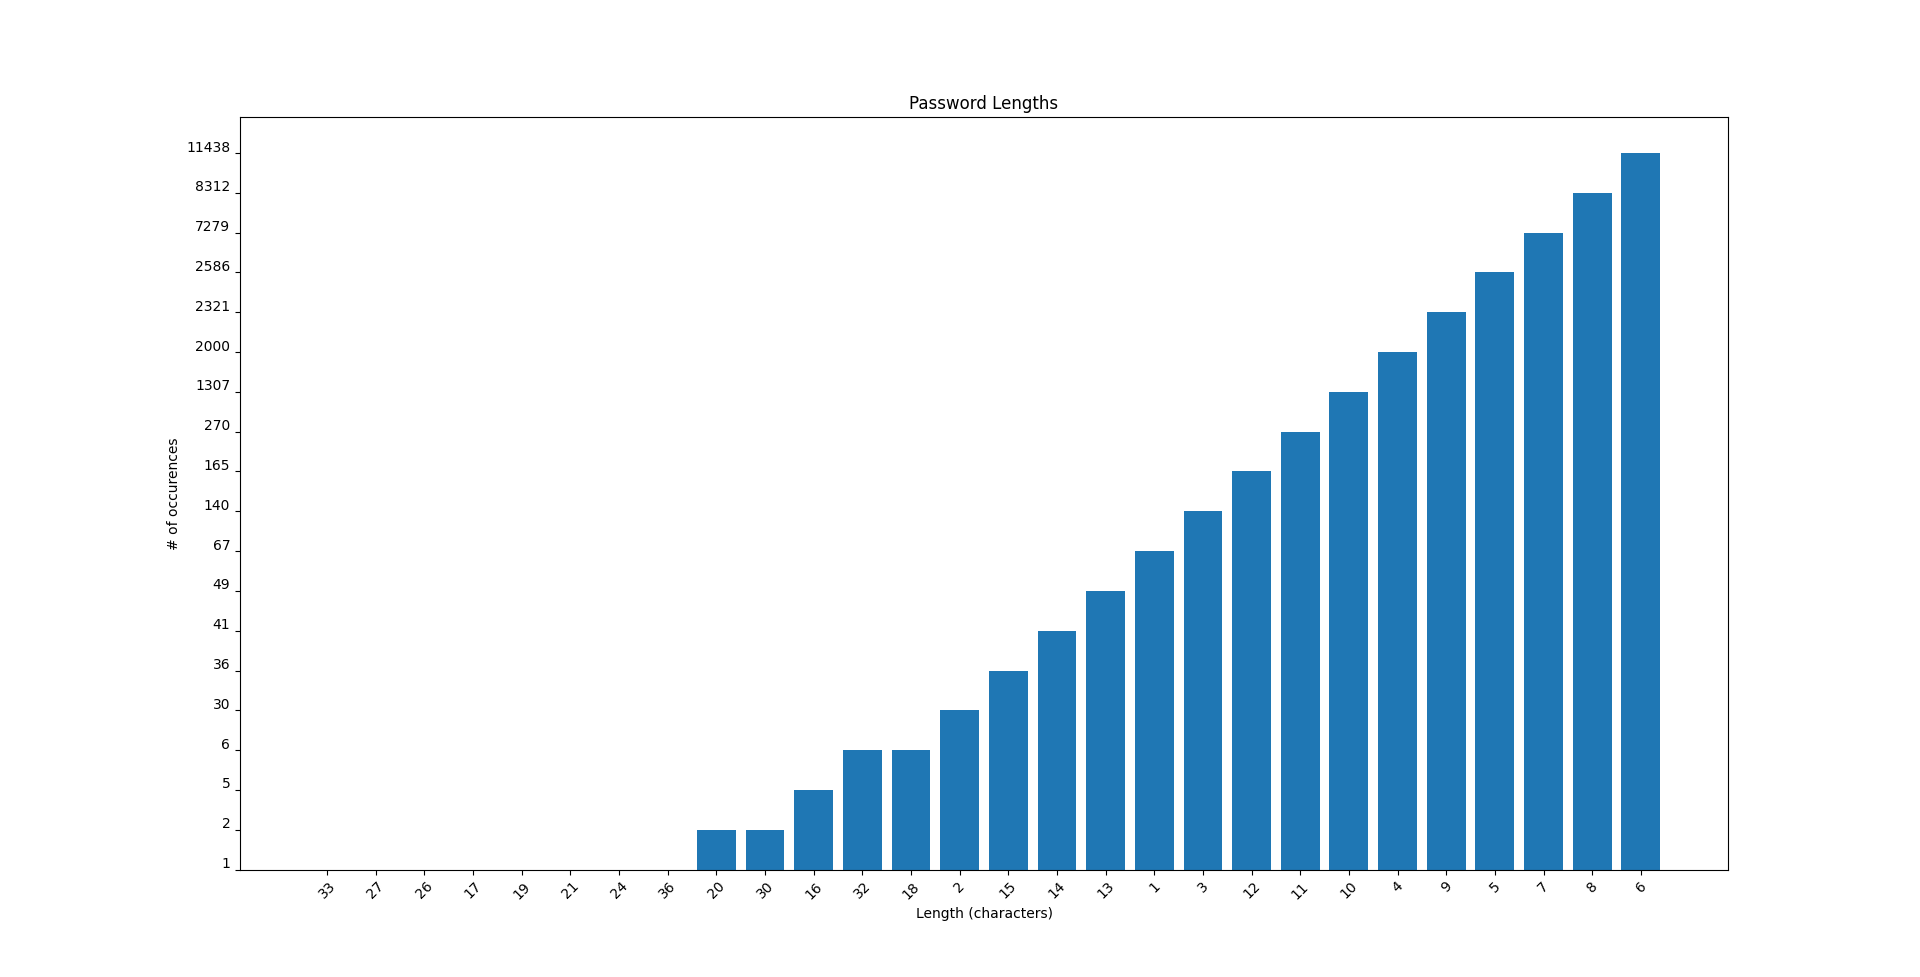
\includegraphics[width=1.8\textwidth]{password_length}
  \caption{Password Length}
  \label{fig:plen}
\end{figure}

\newpage
\subsubsection{What personal information is relevant for password guessing?}

To find the personal information, most relevant for password guessing, one of the password file was analysed manually. The file contained about 10,000 passwords, of which a little over 1,300 were categorised manually, with the help of a simple python script, which can be found in the Appendices (\ref{app:pwordcatscript}). To analyse these passwords, the script parsed over them, after which the researcher decided what category would suit the password best. The researcher then selected or entered the category, after which the script would increment the count on a category or create the category if it did not exist yet. This resulted in a number of categories. Most categories are self-explanatory, which is why not all will be explained in detail. The less evident categories will be handled along with the results.

\begin{figure}[!ht]
  \centering
  \hspace*{-4.3cm}
  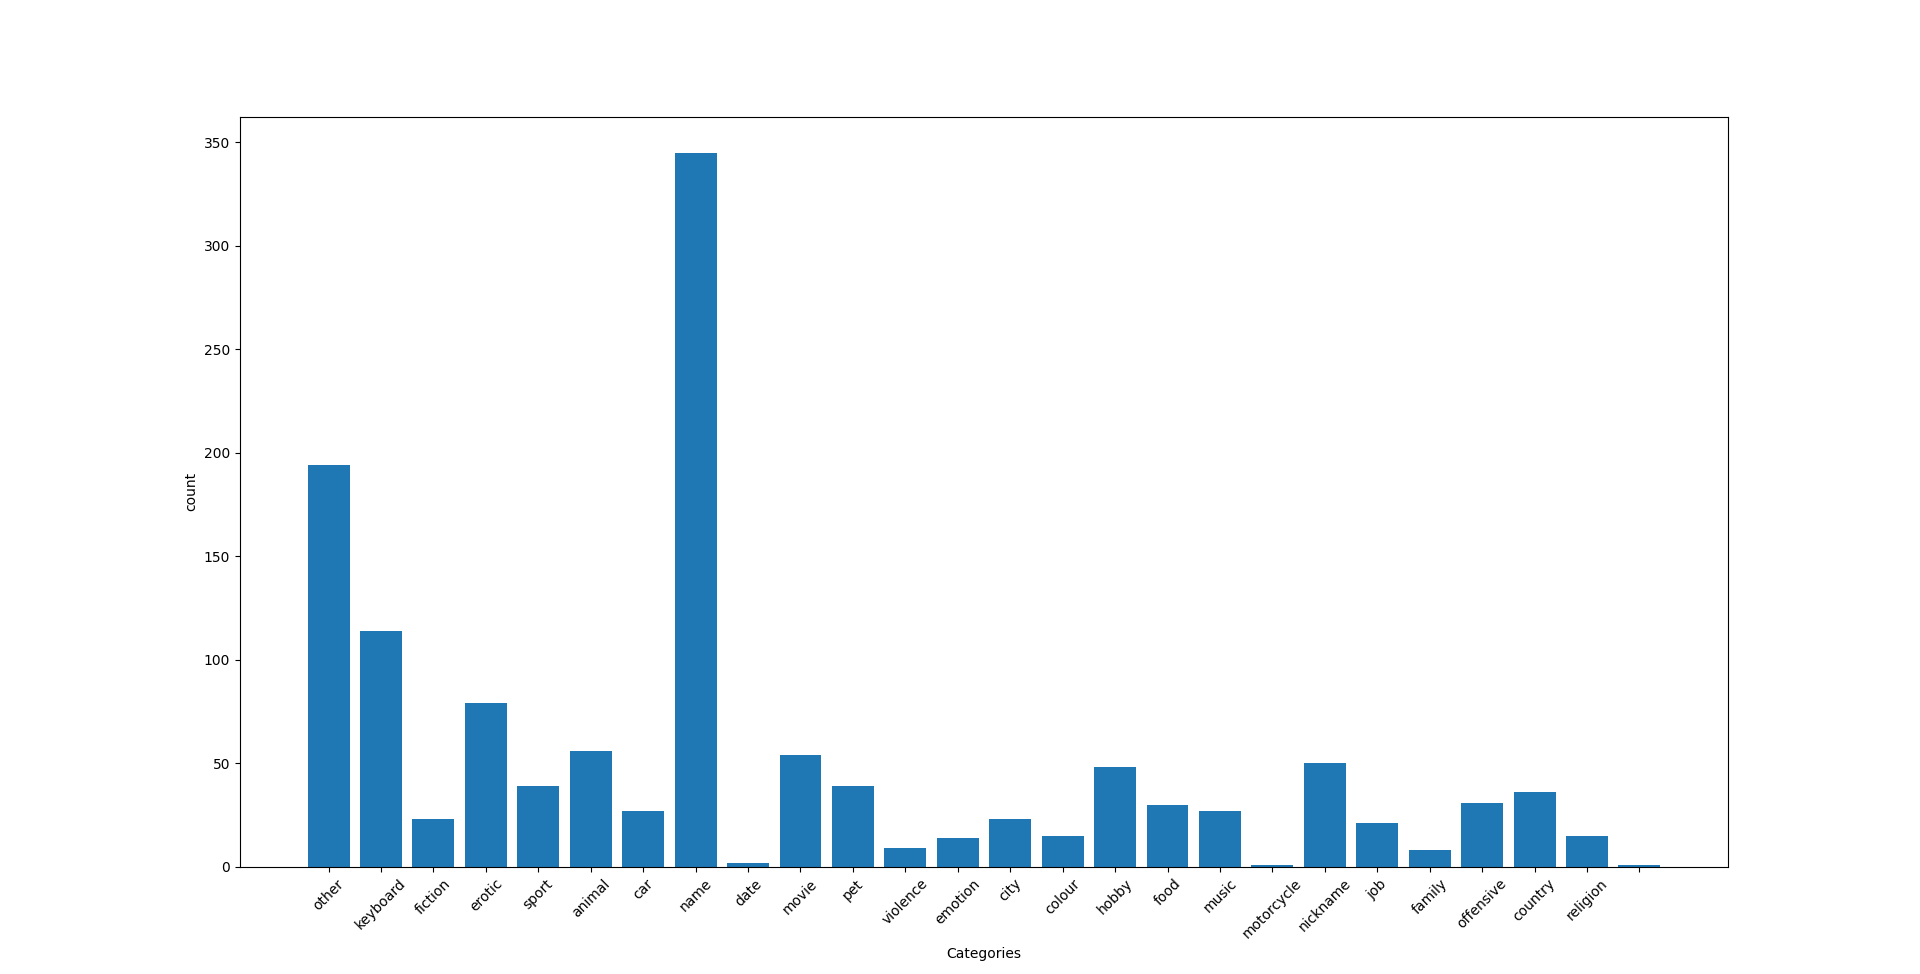
\includegraphics[width=1.7\textwidth]{password_categories}
  \caption{Password Categories}
  \label{fig:pcat}
\end{figure}

The results can be found in figure \ref{fig:pcat}. A number of categories are not entirely self-explanatory, which is why they will be explained in greater detail. The \lstinline{other} category includes all passwords that simply did not fit into any of the others, due to being passwords such as \lstinline{password} or \lstinline{mauyigv68}. Next to this, the \lstinline{keyboard} category can be seen, which hold all passwords that are clearly based on neighbouring keys or otherwise easy keystrokes. Some examples of this are \lstinline{qwerty} and \lstinline{mnbvcxz}.

The results show a large difference between the count of the categories with the \lstinline{name} category being the one with the highest count by far, indicating that this category is important when trying to guess passwords. Since the \lstinline{other} category is a collection of all passwords that did not fit into any category, it is not suprising that this category has a high count. More surprising is the \lstinline{keyboard} category taking the third position, indicating that the patterns that are used for keystroke passwords should be investigated further.\\
The \lstinline{erotic} category also had a large number of passwords, which mostly seemed to have been created jokingly.\\

Other personal information that is often used is sport, like football clubs, baseball clubs, or simply the name of the sport.

\subsubsection{How can the processed information be structured efficiently, to allow for efficient dictionary attacks?}

Since using only the most popular format, with the most popular characters and password length would result in a password such as \lstinline{aaaaaa}, a different approach should be taken. To find the best method for generated passwords to be structured, a number of different approaches are described and compared based on positive and negative aspects.

\begin{itemize}
\item \textit{Generate maximum number of passwords, score passwords and sort according to score.}\\
  This method means to generate as many unique passwords as possible with a list of words, which are related to the target. Based on these words, henceforth called seed words, the program should try and create all possible combinations of the words, common practices, and common replacements of characters. Once this large number of passwords has been created, the passwords should be scored based on the found information. This means that the passwords should be scored for the format they use and how popular this format is, for the characters they use and how popular these characters are, and for the inclusion of words that belong to the found categories. Based on these scores, the passwords should be sorted. The highest scoring passwords should be on the top of the file, with decreasing scores following. This allows dictionary attacks to start with the most probable passwords to be correct. This method is likely to find the right password, as long as the right seed words are provided, although the computational costs are quite significant.\\
    
\item \textit{Generate fewer passwords, aiming specifically at a limited number of formats, score passwords and sort accoring to score.}\\
  This method would generate fewer passwords, but would follow the most popular formats. These passwords would then be scored and sorted much like the previous method. This method would allow for more aimed password generating, although a password would only need a slight deviation from these formats to avoid being guessed. For example, the top 8 formats are all shorter than 12 characters, meaning that a password would avoid being guessed accurately if the password is of a length of 12 or greater and the program only uses the top 8 formats.
\end{itemize}

The first method would be quite computationally heavy and on most systems, would probably take a while to finish. Also, this computation would become exponentially heavy with more seed words, due to more combinations being possible. The second method could be allowed to run much shorter, and could run on far less powerful equipment.\\
On the other hand, the first method will be very likely to generate the accurate password somewhere along the line, as long as the right seed words are provided. The second method will only provide the right password if one of the formats matches the password to be guessed. However, if this smaller list of passwords holds the right password, the increase in speed can be very significant, both when running the wordlist generator and when running a dictionary attack.

\subsubsection{How can the program remain up to date with changing password practices?}


\subsection{Sub-Conclusions}

\begin{itemize}
\item What are standard password formats?

  The results provided valuable information on password formats, password lengths and the most used characters. The results show that passwords, with only lower-case alphabetical characters, a length of six characters, and using the most popular characters such as $a,e,r,o,i,n$, etc. are by far the most used ones. In a more general sense, the most used passwords consist of one type of character, which is either digits or alphabetical characters. Only a fraction of the used password formats mix lower-case alphabetical characters and digits, and a much smaller fraction uses different types of characters, although more than two different types in a single password format was not discovered in the data sets.
  
\item What personal information is relevant for password guessing?

  Looking at the results of categorising passwords, it becomes evident that most passwords are based on names, if based on personal information.
  
\item How can the processed information be structured efficiently, to allow for efficient dictionary attacks?

\item How can the program remain up to date with changing password practices?

\end{itemize}

\newpage
\section{Conclusions}

\newpage
\section{Discussion}

\newpage
\subsection{Recommendations}

\newpage
\begin{thebibliography}{9}
\bibitem{bib:entro}
   Wanli Ma, John Campbell, Dat Tran, Dale Kleeman, Password Entropy and Password Quality, 2010, University of Canberra, Australia \texttt{https://ieeexplore.ieee.org/abstract/document/5635948}
 \bibitem{bib:pform}
   Hsien-Cheng Chou, Hung-Chang Lee, Hwan-Jeu Yu, Fei-Pei Lai, Kuo-Hsuan Huang, Chih-Wen Hsueh, Password Cracking Based On Learned Patterns From Disclosed Passwords, National Taiwan University, New Tapei City, Taiwan \texttt{http://www.ijicic.org/ijicic-11-12068.pdf}
 \bibitem{bib:seclists}
   Daniel Miessler, San Francisco, California, U.S.A \texttt{https://github.com/danielmiessler/SecLists/}
\end{thebibliography}

\newpage
\section{Appendices}

\subsection{Appendix A: SecLists}
\label{app:secl}

SecLists is a collection of data which is freely available on \href{https://github.com/danielmiessler/SecLists/}{Github}. It contains passwords, usernames and much more interesting data which can be used to gain insight in the most used passwords, their formats, used characters and password lengths.

\subsection{Appendix B: Python password format processor}
\label{app:pyprocc}

A Python 3 based script was written to simplify the processing of password data. The script was enabled to parse all data entered as files into a specific directory, splitting the task of processing each file into a separate child process (multiprocessing in Python). 

\begin{lstlisting}[language=Python]
  print('hello world')  
\end{lstlisting}

\subsection{Appendix C: Python graph plotter}
\label{app:pyplot}

To create a new overview for the processed data, a Python script was written to create plots of the data. The script is listed below.

\begin{lstlisting}[language=Python]
  print('hello world')  
\end{lstlisting}

\subsection{Appendix D: Used Password File Names}
\label{app:pwordfile}

\begin{itemize}
\item 10k-most-common.txt
\item probable-v2-top12000.txt
\item unkown-azul.txt
\item clarkson-university-82.txt
\item stupid-ones-in-production.txt
\item darkweb2017-top10000.txt
\item twitter-banned.txt
\end{itemize}

\subsection{Appendix E: Password Categorising Script}
\label{app:pwordcatscript}
\begin{lstlisting}
#!/usr/bin/env python3
import sys
import os
from colorama import Fore, Style
import matplotlib.pyplot as plt

pfile = 'passwords/10k-most-common.txt'
passwords = []

with open(pfile, 'r') as fd:
    lines = fd.readlines()
    for line in lines:
        passwords.append(line.split('\n')[0])

categories = {
}

try:
    for password in passwords:
        print(password)
        index=0
        existing = ''
        for key, value in categories.items():
            existing += ', '+key+'<'+str(index)+'>'
            index += 1
        print('Existing categories:', existing)
        choice = input('Choose category for '+Fore.GREEN+password+Style.RESET_ALL+': ')
        if choice.isdigit():
            print(choice)
            if len(list(categories)) > int(choice):
                key = list(categories)[int(choice)]
                print(key)
            else:
                print('Does not exist yet. Skipping...')
        else:
            key = choice
        if key in categories:
            categories[key] += 1
        else:
            categories[key] = 1
except KeyboardInterrupt:
    print('Making graph')

x = [key for key, value in categories.items()]
y = [value for key, value in categories.items()]

plt.bar(x,y)
plt.xlabel('Categories')
plt.ylabel('count')
plt.xticks(rotation=45)
           
plt.show()
\end{lstlisting}

\end{document}


%%%%%%%%%%%%%%%%%%%%%%%%%%%%%%%%%%%%%%%%%%%%%%%%%%%%%%%%%%%%%%%%%%%%%%%%%%%%%%%%%%%%%%%%%%%%%%%%%%%%%%%%%%%%%%%%%%%%%%%%%%%%%%%%%%%%%%%%%%%%%%%%%%%%%%%%%%%%%%%%%%%%%%%%%%%%%%%%%%%%%%%%%%%%%%%%%%%%%%%%%%%%%%%%%%%%%%%%%%%%%%%%%%%%%%%%%%%%%%%%%%%%%%%%%%%%%%%%%%%%%%%%%%%%%%%%%%%%%%%%%%%%%%%%%%%%%%%%%%%%%%%%%%%%%%%%%%%%%%%%%%%%%%%%%%%%%%%%%%%%%%%%%%%%%%%%%%%%%%%%%%%%%%%%%%%%%%%%%%%%%%%%%%%%%%%%%%%%%%%%%%%%%%%%%%%%%%%%%%%%%%%%%%%%%%%%%%%%%%%%%%%%%%%%%%%%%%%%%%%%%%%%%%%%%%%%%%%%%%%%%%%%%%%%%%%%%%%%%%%%%%%%%%%%%%%%%%%%%%%%%%%%%%%%%%%%%%%%%%%%%%%%%%%%%%%%%%%%%%%%%%%%%%%%%%%%%%%%%%%%%%%%%%%%%%%%%%%%%%%%%%%%%%%%%%%%%%%%%%%%%%%%%%%%%%%%%%%%%%%%%%%%%%%%%%%%%%%%%%%%%%%%%%%%%%%%%%%%%%%%%%%%%%%%%%%%%%%%%%%%%%%%%%%%%%%%%%%%%%%%%%%%%%%%%%%%%%%%%%%%%%%%%%%%%%%%%%%%%%%%%%%%%%%%%%%%%%%%%%%%%%%%%%%%%%%%%%%%%%%%%%%%%%%%%%%%%%%%%%%%%%%%%%%%%%%%%%%%%%%%%%%%%%%%%%%%%%%%%%%%%%%%%%%%%%%%%%%%%%%%%%%%%%%%%%%%%%%%%%%%%%%%%%%%%%%%%%%%%%%%%%%%%%%%%%%%%%%%%%%%%%%%%%
\subsection{Research Results}

The results of the research will be handled per question, firstly dealing with the sub-questions.
The results are listed in this paragraph. The conclusions following this research, will be dealt with in the Conclusions chapter.

\begin{enumerate}
\item \textit{What are standard password formats?}\\
  The first step to answering the sub-question ``\textit{What are standard password formats?}'', was to find useful data to process. For this reason, an online search pointed to the freely available data on Github, called SecLists. A link to this data can be found in the appendices (\ref{app:secl}). This data contains information about frequently used directory names, usernames, passwords and much more. In this research, only the usernames and passwords were relevant and the focus was towards passwords.\\

  The passwords, found in SecLists, were processed with a Python script, which can be found in the appendices (\ref{app:pyprocc}). The script parsed the files placed in the dedicated directory and analysed the format, password length and used characters of each password in the files. 
  

\end{document}
